
%%%%%%%%%%%%%%%%%%%%%%%%%
%%%
%%%%%%%%%%%%%%%%%%%%%%%%%
\begin{frame}\frametitle{Combination of \wbx\ and \htx}
\centering\footnotesize

\begin{minipage}{.5\textwidth}\centering
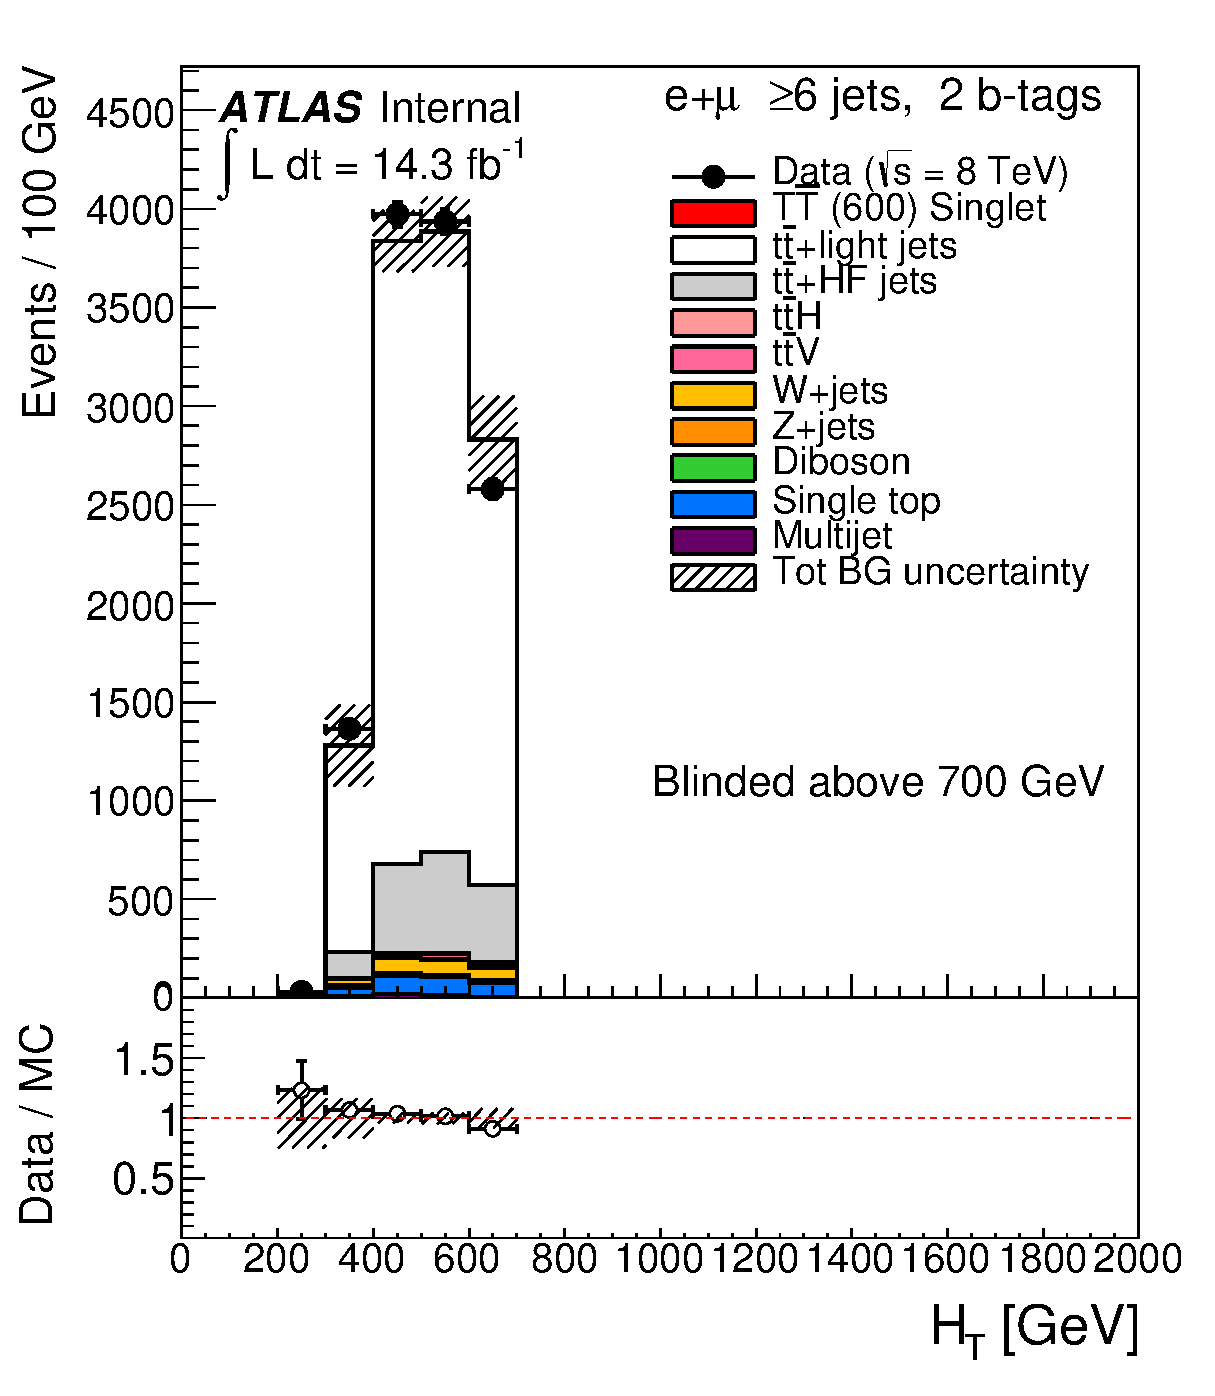
\includegraphics[width=.5\textwidth]{pics/combo/HTAll_6jetin2btagex_ELEMUON}
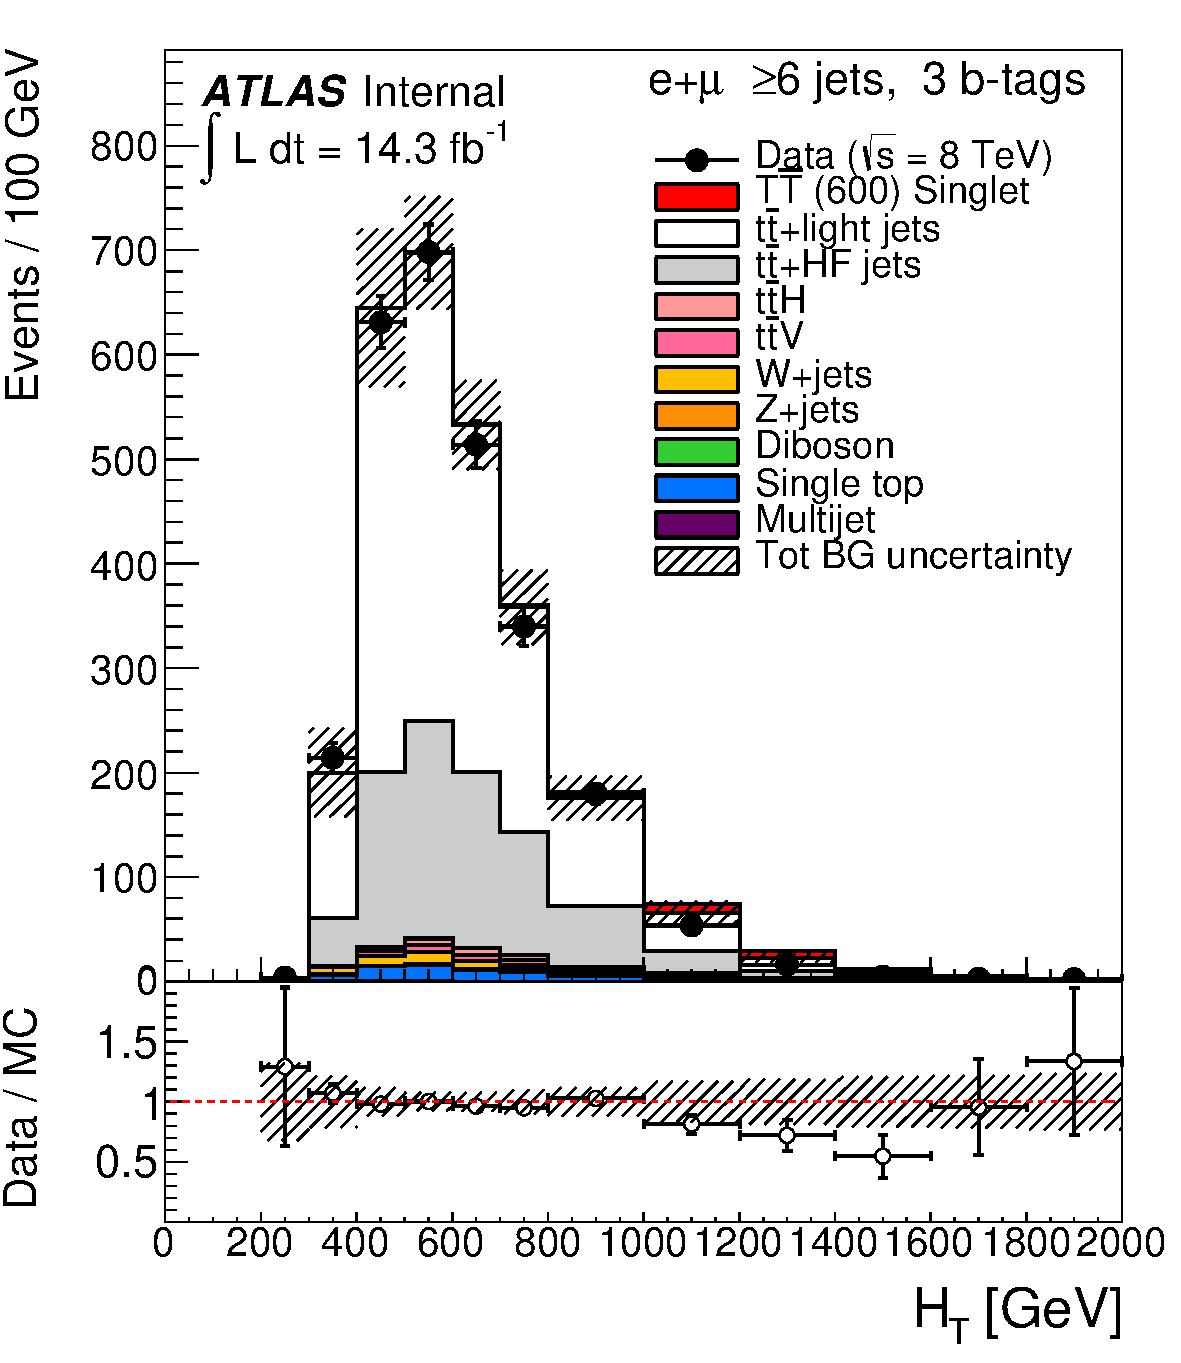
\includegraphics[width=.5\textwidth]{pics/combo/HTAll_6jetin3btagex_ELEMUON}\\
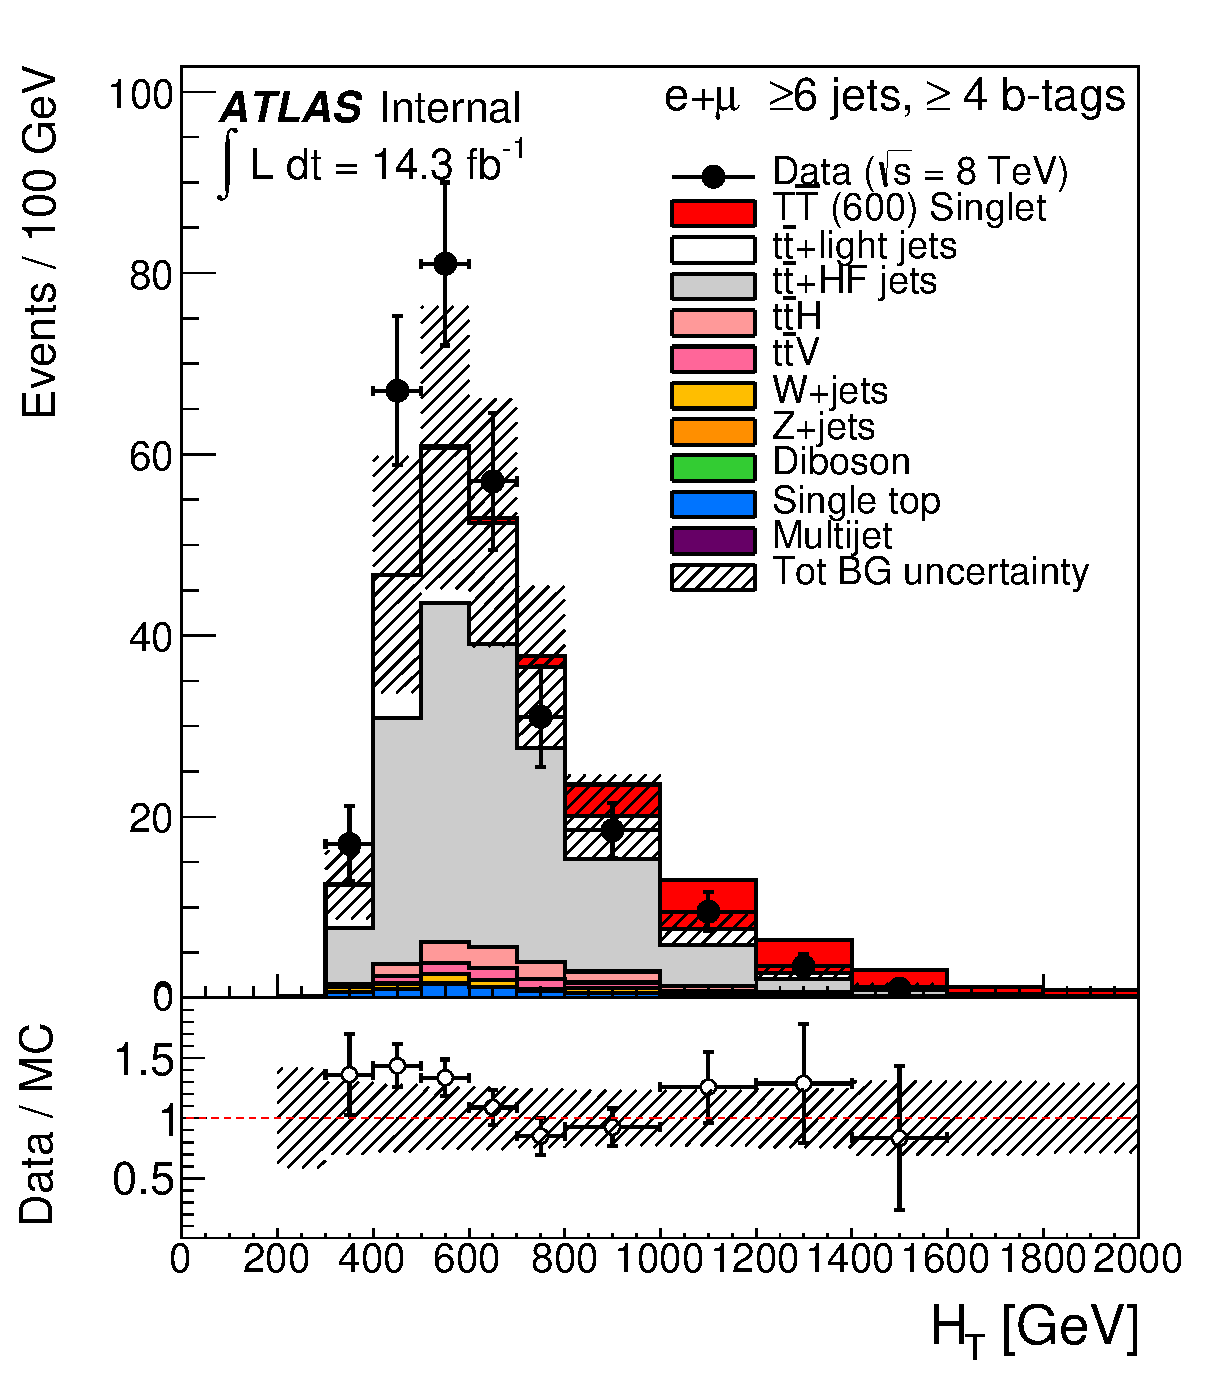
\includegraphics[width=.5\textwidth]{pics/combo/HTAll_6jetin4btagin_ELEMUON}
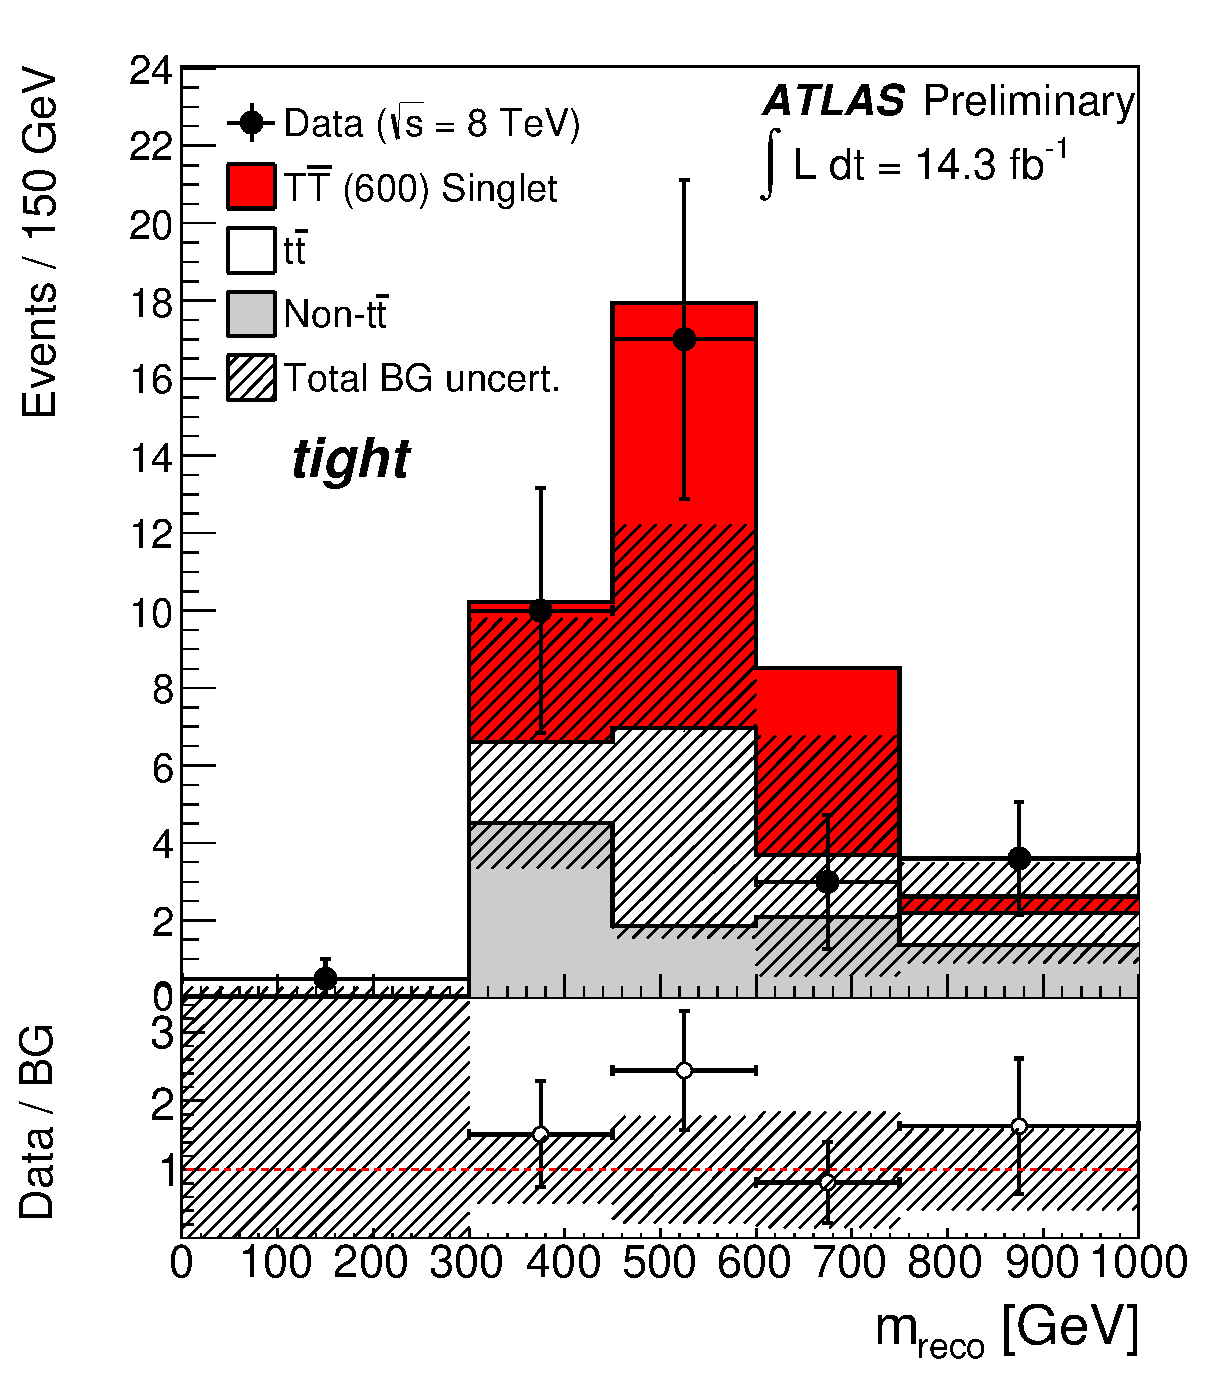
\includegraphics[width=.5\textwidth]{pics/combo/VLQAna_WbX_1W_MWb_4_ELEMUON_cutflow1234567_NOMINAL}

\end{minipage}\begin{minipage}{.5\textwidth}\centering
\myskip

The searches are orthogonal\\
$\Downarrow$\\
can be combined in the statistical analysis\\
(consistent {\cccolor syst unc} treatment)

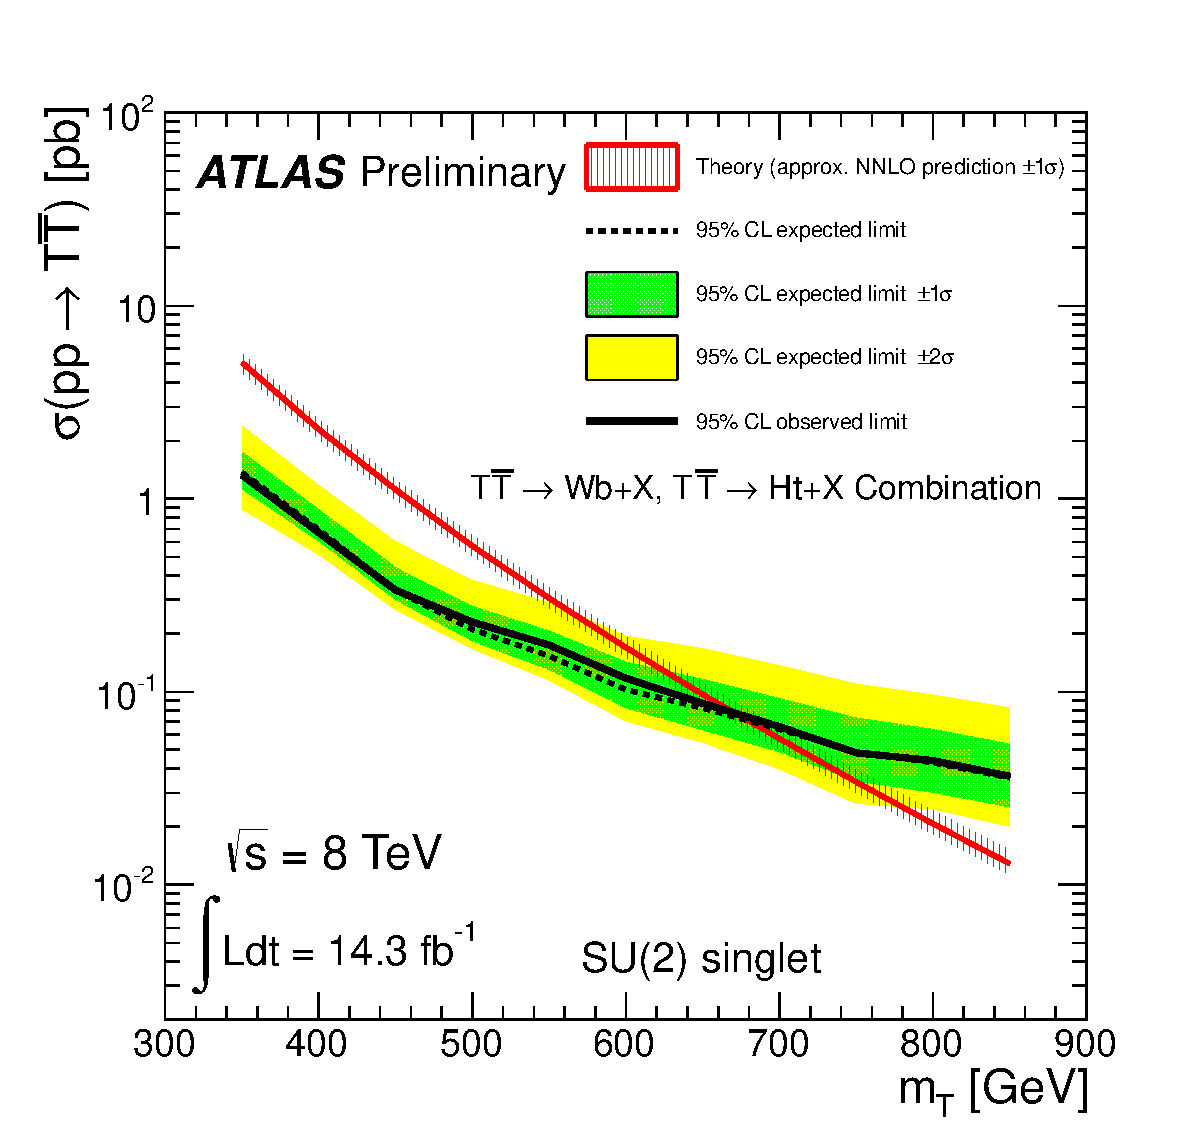
\includegraphics[width=.9\textwidth]{pics/combo/lim_singlet_comb.pdf}

\end{minipage}

\end{frame}



%%%%%%%%%%%%%%%%%%%%%%%%%
%%%
%%%%%%%%%%%%%%%%%%%%%%%%%
\begin{frame}\frametitle{Results}
\centering\footnotesize

\begin{minipage}{.3\textwidth}\centering

aaaa
\end{minipage}\begin{minipage}{.7\textwidth}\centering

\begin{pgfpicture}{0.0\textwidth}{0.0\textheight}{1.\textwidth}{.6\textwidth}
   \begin{pgftranslate}{\pgfpoint{0.0\textwidth}{-0.15\textheight}}
\pgfdeclareimage[interpolate=true,width=1.\textwidth]{wbx}{pics/lim_Scan2D_tight_Bin1.pdf}
\pgfdeclareimage[interpolate=true,width=1.\textwidth]{htx}{pics/combo/htxT.png}
\pgfdeclareimage[interpolate=true,width=1.\textwidth]{comb}{pics/combo/combT.png}
\pgfdeclareimage[interpolate=true,width=1.\textwidth]{br2d}{pics/combo/lim_Scan2D_comb.pdf}
%\pgfputat{\pgfxy(0.0,0.0)}{\pgfbox[left,base]{\pgfuseimage{mindr}}}
 \pgfsetlinewidth{1.pt}
 \usebeamercolor[bg]{head/foot boxes}
\pgfputat{\pgfxy(0.0,0.0)}{\pgfbox[left,base]{\pgfuseimage{wbx}}}
\onslide<2->{
\pgfputat{\pgfxy(0.0,0.0)}{\pgfbox[left,base]{\pgfuseimage{htx}}}
}
\onslide<3->{
\pgfputat{\pgfxy(0.0,0.0)}{\pgfbox[left,base]{\pgfuseimage{comb}}}
}
\onslide<4->{
\pgfputat{\pgfxy(0.0,0.0)}{\pgfbox[left,base]{\pgfuseimage{br2d}}}
}
   \end{pgftranslate}

\end{pgfpicture}

\end{minipage}


\end{frame}

\FullBackgroundPicture{pics/ATLAS_VLQ_TT_june2013_step4}
%%%%%%%%%%%%%%%%%%%%%%%%%
%%%
%%%%%%%%%%%%%%%%%%%%%%%%%
\begin{frame}\frametitle{ATLAS BR coverage}
\centering\footnotesize

%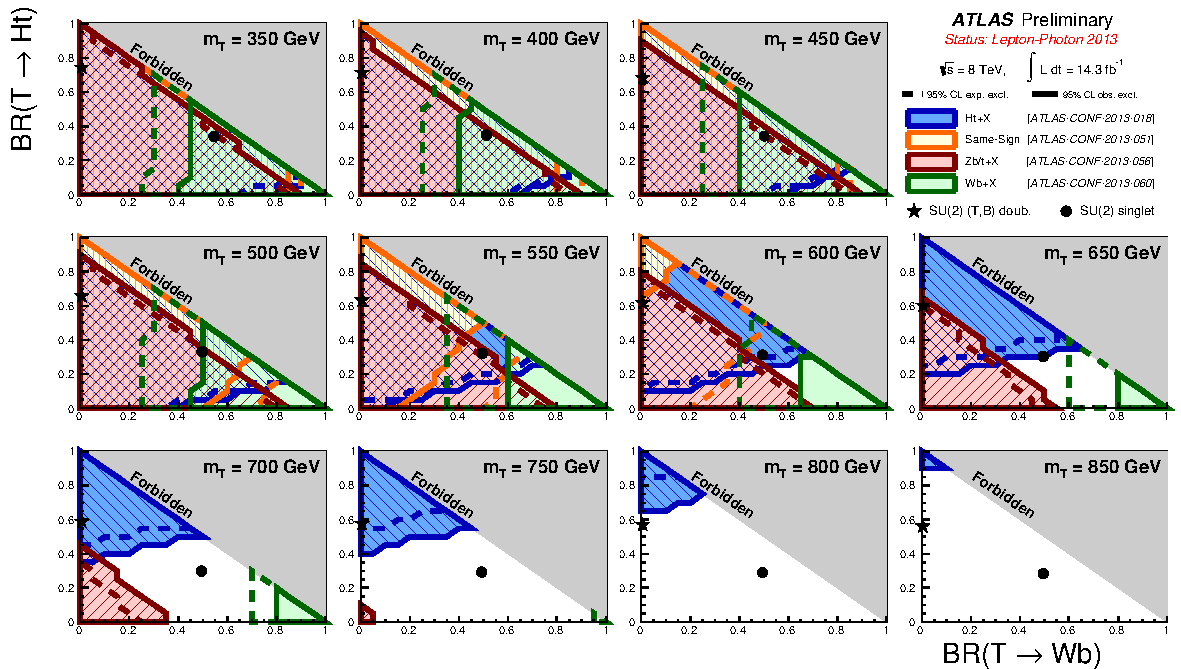
\includegraphics[width=0.8\textwidth]{pics/ATLAS_VLQ_TT_june2013_step4}

\end{frame}


\FullBackgroundPicture{pics/ATLAS_VLQ_BB_june2013_step2}
%%%%%%%%%%%%%%%%%%%%%%%%%
%%%
%%%%%%%%%%%%%%%%%%%%%%%%%
\begin{frame}\frametitle{ATLAS BR coverage}
\centering\footnotesize

%\includegraphics[width=0.8\textwidth]{pics/ATLAS_VLQ_BB_june2013_step2}

\end{frame}


\FullBackgroundPicture{pics/emptyIMG}
%%%%%%%%%%%%%%%%%%%%%%%%%
%%%
%%%%%%%%%%%%%%%%%%%%%%%%%
\begin{frame}\frametitle{Comparison to CMS results}
\centering\footnotesize

Inclusive \TTbar\ searches {\cccolor CMS-PAS-B2G-12-015~\cite{CMS-PAS-B2G-12-015}}
\myskip

\begin{minipage}{.6\textwidth}
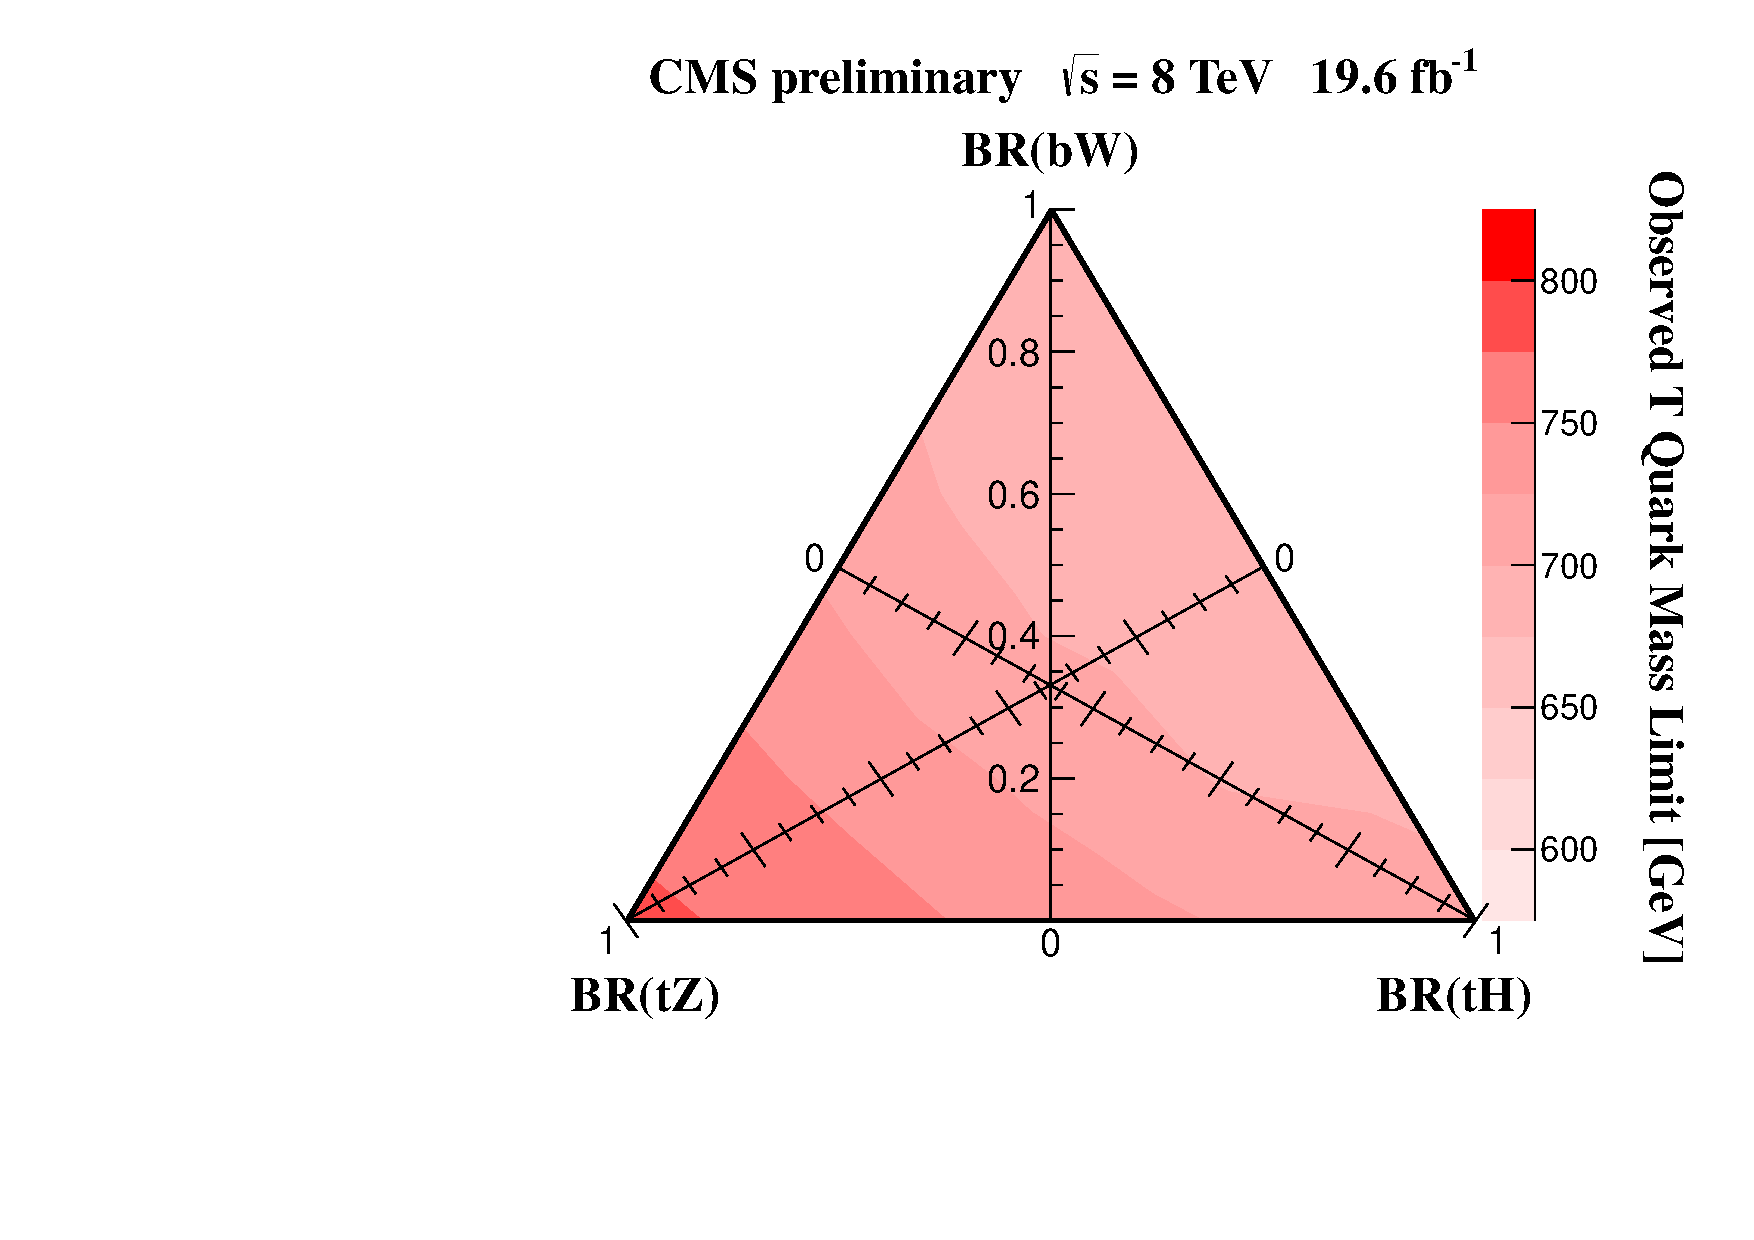
\includegraphics[width=.8\textwidth]{pics/cms/triangle}
\end{minipage}\begin{minipage}{.4\textwidth}\centering

\begin{pgfpicture}{0.0\textwidth}{0.0\textheight}{1.\textwidth}{.6\textwidth}
   \begin{pgftranslate}{\pgfpoint{-0.05\textwidth}{-0.15\textheight}}
\pgfdeclareimage[interpolate=true,width=1.\textwidth]{tabTT}{pics/cms/tableTT}
 \pgfsetlinewidth{1.pt}
 \usebeamercolor[bg]{head/foot boxes}
 \pgfputat{\pgfxy(0.0,0.0)}{\pgfbox[left,base]{\pgfuseimage{tabTT}}}
 \pgfrect[stroke]{\pgfxy(0.2,3.4)}{\pgfxy(5,0.25)}
 \pgfputat{\pgfxy(-1.2,3.4)}{\pgfbox[left,base]{\cccolor ``doublet''}}
 \pgfputat{\pgfxy(-1.2,3.1)}{\pgfbox[left,base]{\cccolor 790 obs}}
 \pgfrect[stroke]{\pgfxy(0.2,1.4)}{\pgfxy(5,0.25)}
 \pgfputat{\pgfxy(-1.2,1.4)}{\pgfbox[left,base]{\cccolor ``singlet''}}
 \pgfputat{\pgfxy(-1.2,1.1)}{\pgfbox[left,base]{\cccolor 670 obs}}
 \pgfrect[stroke]{\pgfxy(0.2,0.)}{\pgfxy(5,0.25)}
 \pgfputat{\pgfxy(-1.2,0.)}{\pgfbox[left,base]{\cccolor ``chiral''}}
 \pgfputat{\pgfxy(-1.2,-0.3)}{\pgfbox[left,base]{\cccolor 740 obs}}
 \pgfrect[stroke]{\pgfxy(4,-0.05)}{\pgfxy(1,5.)}
\end{pgftranslate}
\end{pgfpicture}

\end{minipage}


\end{frame}



